
%(BEGIN_QUESTION)
% Copyright 2011, Tony R. Kuphaldt, released under the Creative Commons Attribution License (v 1.0)
% This means you may do almost anything with this work of mine, so long as you give me proper credit

Denne varmevekslerens utløpstemperatur reguleres av en PID-kontroller som styrer hvor mye damp som slipper inn i veksleren for å varme prosessvæsken:

$$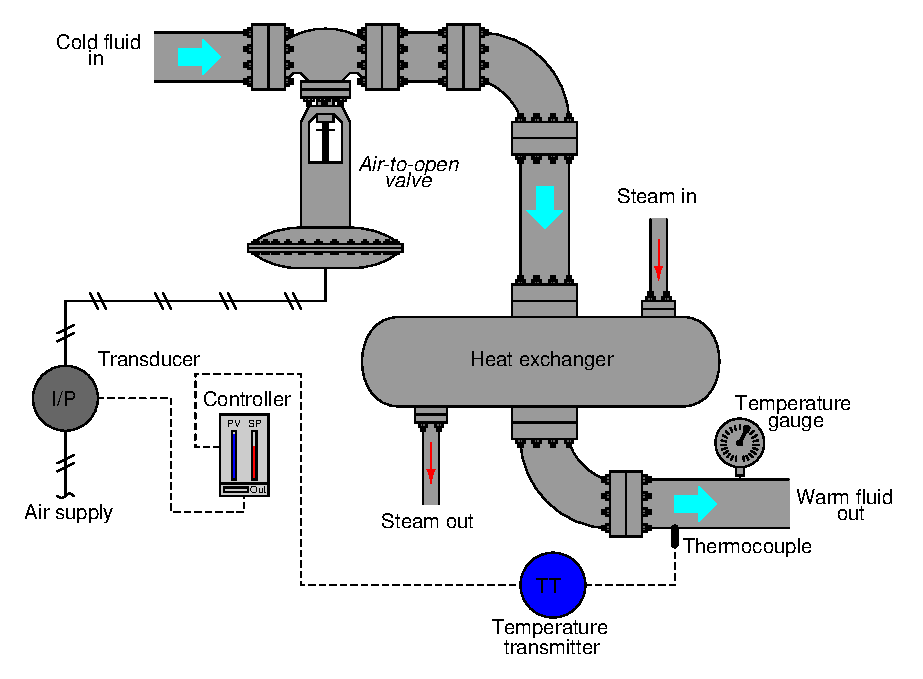
\includegraphics[width=15.5cm]{i00297x01.eps}$$

En operatør sier systemet har et problem: kontrollerens frontpanel viser temperatur godt over settpunkt.  Du ser samtidig at stolpediagrammet for utgang på frontpanelet står på 0\%.  En annen operatør ute i felt (ved veksleren) melder over radio at reguleringsventilstammen står i ``lukket'' posisjon.

\vskip 10pt

En annen instrumenttekniker ved siden av deg anbefaler å sette kontrolleren i manuell modus for en rask slagtest av reguleringsventilen (verifisere respons på kontrollerutgang).  Forklar hvorfor denne testen ville vært bortkastet tid, og foreslå en bedre test for å snevre inn feilplasseringen.

\vskip 20pt \vbox{\hrule \hbox{\strut \vrule{} {\bf Forslag til sokratisk diskusjon} \vrule} \hrule}

\begin{itemize}
\item{} Et nyttig prinsipp i en diagnostisk situasjon som denne er \textit{correspondence}: identifiser hvilke feltvariabler som samsvarer med kontrollerens frontpanelvisning, og hvilke som ikke gjør det.  Bruk denne sammenligningen til å forklare hvorfor teknikerens forslag sannsynligvis ikke var beste første steg.
\end{itemize}

\underbar{file i00297}
%(END_QUESTION)





%(BEGIN_ANSWER)

Grunnen til at den foreslåtte testen ville vært bortkastet, er at reguleringsventilen allerede gjør det kontrolleren ber den om: gå til 0\% (lukket).  Ventilstammens posisjon samsvarer altså med kontrollerens utgangsindikasjon, noe som tyder på at det ikke er feil i den (utgangs-)delen av reguleringssystemet.

\vskip 10pt

Kontrollerens ``beslutning'' om å stenge ventilen gir ikke mening ut fra PV $>$ SP.  Det kontrolleren burde gjøre er å åpne kaldmatingsventilen for å redusere prosesstemperaturen.  Vi vet ikke om PV-indikasjonen samsvarer med temperaturmåleren, men det er faktisk mindre viktig akkurat nå fordi vi vet sikkert at kontrolleren ikke tar riktig handling for det den ``ser'' av PV og SP.  Mulige feil er:

\begin{itemize}
\item{} Kontrolleren står i manuell modus (ikke auto)
\item{} Svært dårlig regulator-tuning
\item{} Feil kontrollerretning (action)
\end{itemize}

Et godt neste steg er å sjekke om kontrolleren står i automatisk modus.  Hvis den gjør det, ligger feilen i kontrollerens konfigurasjon eller tuning.

%(END_ANSWER)





%(BEGIN_NOTES)


%INDEX% Basics, control loop troubleshooting: isolating area of fault by correspondence

%(END_NOTES)
